\documentclass[tikz,border=8pt]{standalone}
\usepackage[utf8]{inputenc}
\usepackage{lmodern}
\usepackage[T1]{fontenc}
\usepackage{amsmath,amssymb}
\usetikzlibrary{shapes.geometric, arrows.meta, positioning, calc, fit, backgrounds}

\definecolor{tealA}{HTML}{0D7377}
\definecolor{tealB}{HTML}{14919B}
\definecolor{tealC}{HTML}{E0F7F7}
\definecolor{amberA}{HTML}{D97706}
\definecolor{amberC}{HTML}{FEF3C7}
\definecolor{slateG}{HTML}{475569}

\begin{document}
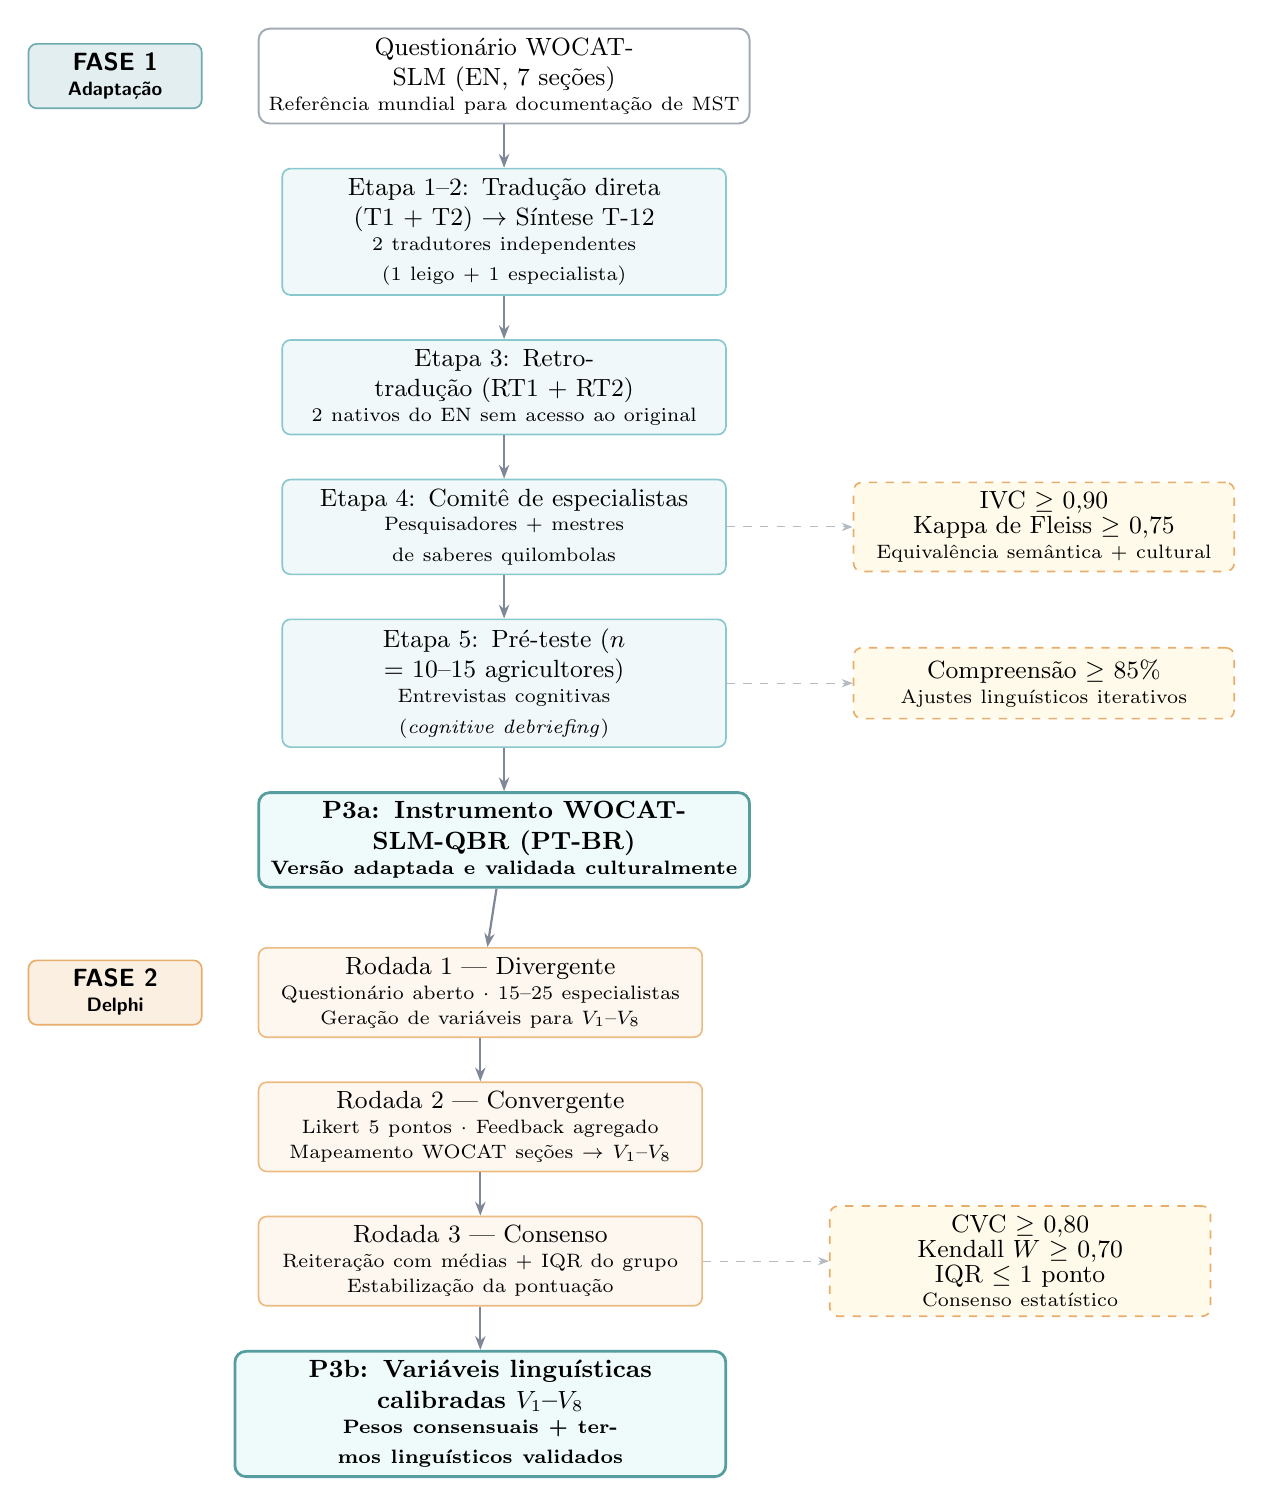
\begin{tikzpicture}[
  phase/.style={
    fill=#1!12, draw=#1!60,
    font=\sffamily\bfseries\small,
    minimum width=2.2cm, minimum height=0.8cm,
    align=center, rounded corners=3pt,
    line width=0.6pt
  },
  mainbox/.style={
    draw=slateG!50, fill=white,
    font=\small, align=center,
    minimum width=6.2cm, minimum height=1.0cm,
    rounded corners=4pt, text width=6.0cm,
    line width=0.7pt
  },
  stepbox/.style={
    draw=#1!50, fill=#1!6,
    font=\small, align=center,
    minimum width=5.6cm, minimum height=0.9cm,
    rounded corners=3pt, text width=5.4cm,
    line width=0.6pt
  },
  metricbox/.style={
    draw=amberA!60, fill=amberC!40,
    font=\small, align=center,
    minimum width=4.8cm, minimum height=0.9cm,
    rounded corners=3pt, text width=4.6cm,
    line width=0.6pt, dashed
  },
  outputbox/.style={
    draw=tealA!70, fill=tealC!50,
    font=\small\bfseries, align=center,
    minimum width=6.2cm, minimum height=1.0cm,
    rounded corners=4pt, text width=6.0cm,
    line width=1pt
  },
  arr/.style={-{Stealth[length=5pt]}, thick, slateG!70},
  darr/.style={-{Stealth[length=4pt]}, thin, slateG!40, dashed},
  node distance=0.55cm
]

%% ═══ FASE 1 — ADAPTAÇÃO TRANSCULTURAL (Beaton) ═══
\node[phase=tealA] (ph1) {FASE 1\\[-2pt]{\scriptsize Adapta\c{c}\~ao}};

\node[mainbox, right=0.7cm of ph1] (input)
  {Question\'ario WOCAT-SLM (EN, 7 se\c{c}\~oes)\\[-2pt]
   {\scriptsize Refer\^encia mundial para documenta\c{c}\~ao de MST}};

\node[stepbox=tealB, below=of input] (t1)
  {Etapa 1--2: Tradu\c{c}\~ao direta (T1 + T2) $\rightarrow$ S\'{\i}ntese T-12\\[-2pt]
   {\scriptsize 2 tradutores independentes (1 leigo + 1 especialista)}};
\draw[arr] (input) -- (t1);

\node[stepbox=tealB, below=of t1] (rt)
  {Etapa 3: Retrotradu\c{c}\~ao (RT1 + RT2)\\[-2pt]
   {\scriptsize 2 nativos do EN sem acesso ao original}};
\draw[arr] (t1) -- (rt);

\node[stepbox=tealB, below=of rt] (comite)
  {Etapa 4: Comit\^e de especialistas\\[-2pt]
   {\scriptsize Pesquisadores + mestres de saberes quilombolas}};
\draw[arr] (rt) -- (comite);

\node[metricbox, right=1.6cm of comite] (ivc)
  {IVC $\geq$ 0{,}90\\[-2pt]
   Kappa de Fleiss $\geq$ 0{,}75\\[-2pt]
   {\scriptsize Equival\^encia sem\^antica + cultural}};
\draw[darr] (comite) -- (ivc);

\node[stepbox=tealB, below=of comite] (preteste)
  {Etapa 5: Pr\'e-teste ($n$ = 10--15 agricultores)\\[-2pt]
   {\scriptsize Entrevistas cognitivas (\textit{cognitive debriefing})}};
\draw[arr] (comite) -- (preteste);

\node[metricbox, right=1.6cm of preteste] (comp)
  {Compreens\~ao $\geq$ 85\%\\[-2pt]
   {\scriptsize Ajustes lingu\'{\i}sticos iterativos}};
\draw[darr] (preteste) -- (comp);

\node[outputbox, below=of preteste] (p3a)
  {P3a: Instrumento WOCAT-SLM-QBR (PT-BR)\\[-2pt]
   {\scriptsize Vers\~ao adaptada e validada culturalmente}};
\draw[arr] (preteste) -- (p3a);

%% ═══ FASE 2 — DELPHI ═══
\node[phase=amberA, below=0.9cm of ph1 |- p3a.south] (ph2)
  {FASE 2\\[-2pt]{\scriptsize Delphi}};

\node[stepbox=amberA, right=0.7cm of ph2] (r1)
  {Rodada 1 --- Divergente\\[-2pt]
   {\scriptsize Question\'ario aberto $\cdot$ 15--25 especialistas}\\[-2pt]
   {\scriptsize Gera\c{c}\~ao de vari\'aveis para $V_1$--$V_8$}};
\draw[arr] (p3a) -- (r1);

\node[stepbox=amberA, below=of r1] (r2)
  {Rodada 2 --- Convergente\\[-2pt]
   {\scriptsize Likert 5 pontos $\cdot$ Feedback agregado}\\[-2pt]
   {\scriptsize Mapeamento WOCAT se\c{c}\~oes $\rightarrow$ $V_1$--$V_8$}};
\draw[arr] (r1) -- (r2);

\node[stepbox=amberA, below=of r2] (r3)
  {Rodada 3 --- Consenso\\[-2pt]
   {\scriptsize Reitera\c{c}\~ao com m\'edias + IQR do grupo}\\[-2pt]
   {\scriptsize Estabiliza\c{c}\~ao da pontua\c{c}\~ao}};
\draw[arr] (r2) -- (r3);

\node[metricbox, right=1.6cm of r3] (wk)
  {CVC $\geq$ 0{,}80\\[-2pt]
   Kendall $W$ $\geq$ 0{,}70\\[-2pt]
   IQR $\leq$ 1 ponto\\[-2pt]
   {\scriptsize Consenso estat\'{\i}stico}};
\draw[darr] (r3) -- (wk);

\node[outputbox, below=of r3] (p3b)
  {P3b: Vari\'aveis lingu\'{\i}sticas calibradas $V_1$--$V_8$\\[-2pt]
   {\scriptsize Pesos consensuais + termos lingu\'{\i}sticos validados}};
\draw[arr] (r3) -- (p3b);

\end{tikzpicture}
\end{document}
